\documentclass{standalone}
\usepackage{tikz}
\usetikzlibrary{patterns, positioning}
\usepackage[sfdefault]{ClearSans} %% option 'sfdefault' activates Clear Sans as the default text font
\usepackage[T1]{fontenc}

\begin{document}
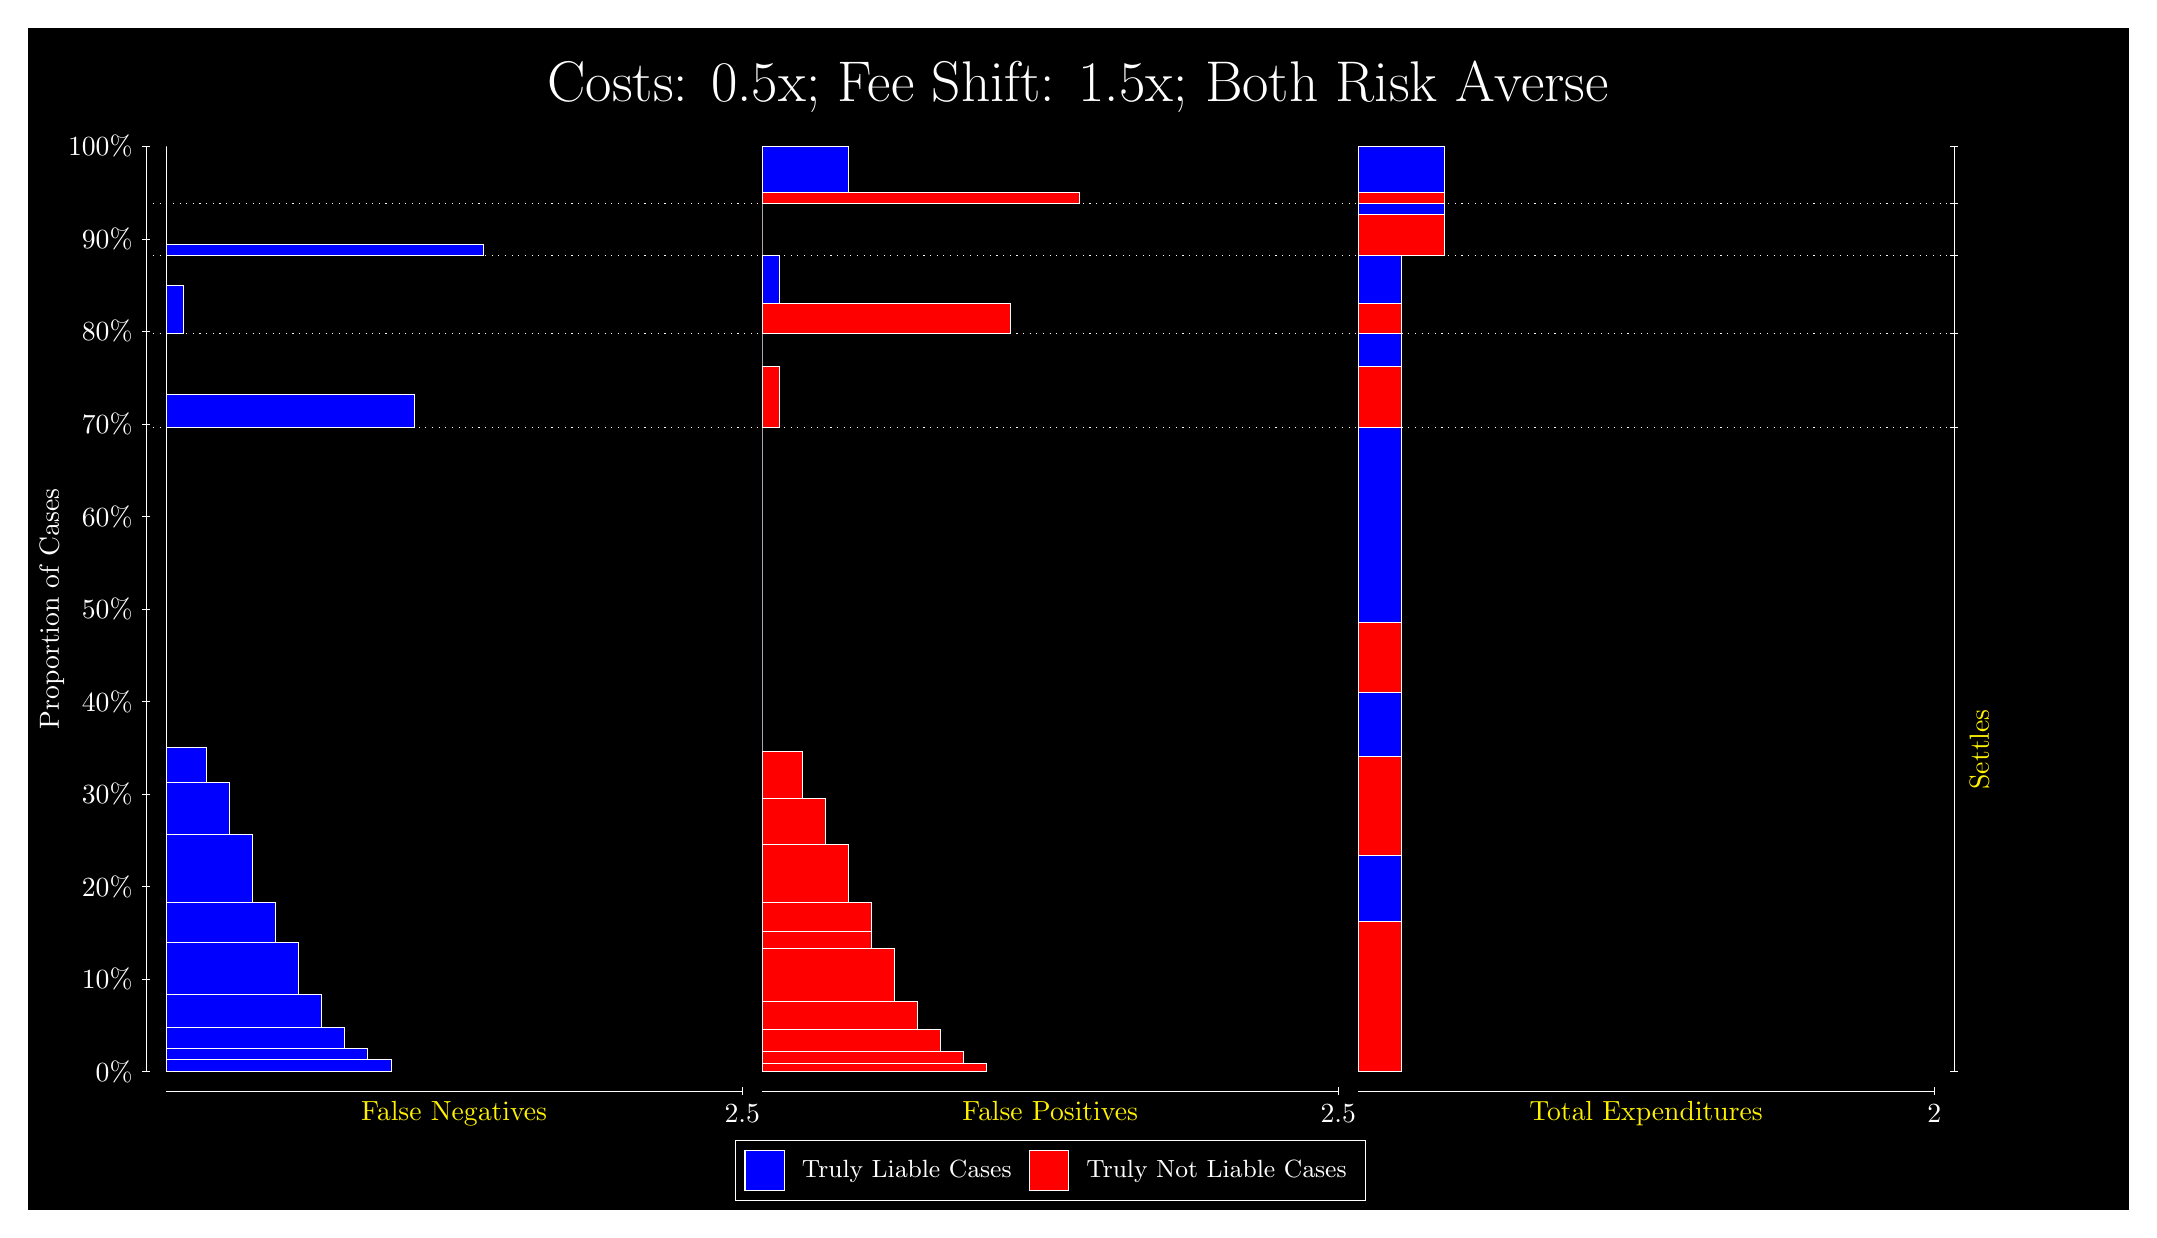
\begin{tikzpicture}
\draw[fill=black] (0,0) rectangle (26.667,15);
\draw[text=white] (0,13.5) rectangle (26.667,15) node[midway] {\huge Costs: 0.5x; Fee Shift: 1.5x; Both Risk Averse};
\draw[white, very thin] (1.5,1.75) -- (1.5,13.5);
\node[rotate=90, text=white, anchor=center] at (0.3, 7.625) {Proportion of Cases};
\draw[white, very thin] (1.45,1.75) -- (1.55,1.75);
\node[text=white, anchor=east] at (1.45, 1.75) {0\%};
\draw[white, very thin] (1.45,2.925) -- (1.55,2.925);
\node[text=white, anchor=east] at (1.45, 2.925) {10\%};
\draw[white, very thin] (1.45,4.1) -- (1.55,4.1);
\node[text=white, anchor=east] at (1.45, 4.1) {20\%};
\draw[white, very thin] (1.45,5.275) -- (1.55,5.275);
\node[text=white, anchor=east] at (1.45, 5.275) {30\%};
\draw[white, very thin] (1.45,6.45) -- (1.55,6.45);
\node[text=white, anchor=east] at (1.45, 6.45) {40\%};
\draw[white, very thin] (1.45,7.625) -- (1.55,7.625);
\node[text=white, anchor=east] at (1.45, 7.625) {50\%};
\draw[white, very thin] (1.45,8.8) -- (1.55,8.8);
\node[text=white, anchor=east] at (1.45, 8.8) {60\%};
\draw[white, very thin] (1.45,9.975) -- (1.55,9.975);
\node[text=white, anchor=east] at (1.45, 9.975) {70\%};
\draw[white, very thin] (1.45,11.15) -- (1.55,11.15);
\node[text=white, anchor=east] at (1.45, 11.15) {80\%};
\draw[white, very thin] (1.45,12.325) -- (1.55,12.325);
\node[text=white, anchor=east] at (1.45, 12.325) {90\%};
\draw[white, very thin] (1.45,13.5) -- (1.55,13.5);
\node[text=white, anchor=east] at (1.45, 13.5) {100\%};

\draw[white, very thin] (24.457,1.75) -- (24.457,13.5);
\draw[white, very thin] (24.407,1.75) -- (24.507,1.75);
\node[anchor=west] at (24.407, 1.75) {};
\draw[white, very thin] (24.407,9.9331) -- (24.507,9.9331);
\node[anchor=west] at (24.407, 9.9331) {};
\draw[white, very thin] (24.407,11.122) -- (24.507,11.122);
\node[anchor=west] at (24.407, 11.122) {};
\draw[white, very thin] (24.407,12.119) -- (24.507,12.119);
\node[anchor=west] at (24.407, 12.119) {};
\draw[white, very thin] (24.407,12.778) -- (24.507,12.778);
\node[anchor=west] at (24.407, 12.778) {};
\draw[white, very thin] (24.407,13.5) -- (24.507,13.5);
\node[anchor=west] at (24.407, 13.5) {};

\draw[white, very thin, fill=blue] (1.75,1.75) rectangle (4.6044,1.8996);
\draw[white, very thin, fill=blue] (1.75,1.8996) rectangle (4.3116,2.0483);
\draw[white, very thin, fill=blue] (1.75,2.0483) rectangle (4.0188,2.3106);
\draw[white, very thin, fill=blue] (1.75,2.3106) rectangle (3.7261,2.7317);
\draw[white, very thin, fill=blue] (1.75,2.7317) rectangle (3.4333,3.3947);
\draw[white, very thin, fill=blue] (1.75,3.3947) rectangle (3.1406,3.9031);
\draw[white, very thin, fill=blue] (1.75,3.9031) rectangle (2.8478,4.7599);
\draw[white, very thin, fill=blue] (1.75,4.7599) rectangle (2.5551,5.4184);
\draw[white, very thin, fill=blue] (1.75,5.4184) rectangle (2.2623,5.8705);
\draw[white, very thin, fill=red] (1.75,5.8705) rectangle (1.75,9.9331);
\draw[white, very thin, fill=blue] (1.75,9.9331) rectangle (4.8971,10.35);
\draw[white, very thin, fill=red] (1.75,10.35) rectangle (1.75,11.122);
\draw[white, very thin, fill=blue] (1.75,11.122) rectangle (1.9696,11.738);
\draw[white, very thin, fill=red] (1.75,11.738) rectangle (1.75,12.119);
\draw[white, very thin, fill=blue] (1.75,12.119) rectangle (5.7754,12.258);
\draw[white, very thin, fill=red] (1.75,12.258) rectangle (1.75,12.778);
\draw[white, very thin, fill=red] (1.75,12.778) rectangle (1.75,12.918);
\draw[white, very thin, fill=blue] (1.75,12.918) rectangle (1.75,13.5);
\draw[white, very thin, fill=red] (9.3189,1.75) rectangle (12.173,1.8589);
\draw[white, very thin, fill=red] (9.3189,1.8589) rectangle (11.88,2.0049);
\draw[white, very thin, fill=red] (9.3189,2.0049) rectangle (11.588,2.2823);
\draw[white, very thin, fill=red] (9.3189,2.2823) rectangle (11.295,2.6435);
\draw[white, very thin, fill=red] (9.3189,2.6435) rectangle (11.002,3.3115);
\draw[white, very thin, fill=red] (9.3189,3.3115) rectangle (10.709,3.5317);
\draw[white, very thin, fill=red] (9.3189,3.5317) rectangle (10.709,3.9002);
\draw[white, very thin, fill=red] (9.3189,3.9002) rectangle (10.417,4.6409);
\draw[white, very thin, fill=red] (9.3189,4.6409) rectangle (10.124,5.2251);
\draw[white, very thin, fill=red] (9.3189,5.2251) rectangle (9.8312,5.8126);
\draw[white, very thin, fill=blue] (9.3189,5.8126) rectangle (9.3189,9.9331);
\draw[white, very thin, fill=red] (9.3189,9.9331) rectangle (9.5384,10.705);
\draw[white, very thin, fill=blue] (9.3189,10.705) rectangle (9.3189,11.122);
\draw[white, very thin, fill=red] (9.3189,11.122) rectangle (12.466,11.502);
\draw[white, very thin, fill=blue] (9.3189,11.502) rectangle (9.5384,12.119);
\draw[white, very thin, fill=red] (9.3189,12.119) rectangle (9.3189,12.639);
\draw[white, very thin, fill=blue] (9.3189,12.639) rectangle (9.3189,12.778);
\draw[white, very thin, fill=red] (9.3189,12.778) rectangle (13.344,12.918);
\draw[white, very thin, fill=blue] (9.3189,12.918) rectangle (10.417,13.5);
\draw[white, very thin, fill=red] (16.888,1.75) rectangle (17.437,3.6637);
\draw[white, very thin, fill=blue] (16.888,3.6637) rectangle (17.437,4.4958);
\draw[white, very thin, fill=red] (16.888,4.4958) rectangle (17.437,5.7512);
\draw[white, very thin, fill=blue] (16.888,5.7512) rectangle (17.437,6.5638);
\draw[white, very thin, fill=red] (16.888,6.5638) rectangle (17.437,7.4573);
\draw[white, very thin, fill=blue] (16.888,7.4573) rectangle (17.437,9.9331);
\draw[white, very thin, fill=red] (16.888,9.9331) rectangle (17.437,10.705);
\draw[white, very thin, fill=blue] (16.888,10.705) rectangle (17.437,11.122);
\draw[white, very thin, fill=red] (16.888,11.122) rectangle (17.437,11.502);
\draw[white, very thin, fill=blue] (16.888,11.502) rectangle (17.437,12.119);
\draw[white, very thin, fill=red] (16.888,12.119) rectangle (17.986,12.639);
\draw[white, very thin, fill=blue] (16.888,12.639) rectangle (17.986,12.778);
\draw[white, very thin, fill=red] (16.888,12.778) rectangle (17.986,12.918);
\draw[white, very thin, fill=blue] (16.888,12.918) rectangle (17.986,13.5);
\draw[white, dotted] (1.5,9.9331) -- (24.457,9.9331);
\draw[white, dotted] (1.5,11.122) -- (24.457,11.122);
\draw[white, dotted] (1.5,12.119) -- (24.457,12.119);
\draw[white, dotted] (1.5,12.778) -- (24.457,12.778);
\draw[white, very thin] (1.75,1.5) -- (9.0689,1.5);
\node[text=yellow, anchor=north] at (5.4094, 1.5) {False Negatives};
\draw[white, very thin] (9.0689,1.45) -- (9.0689,1.55);
\node[text=white, anchor=north] at (9.0689, 1.45) {2.5};

\draw[white, very thin] (9.3189,1.5) -- (16.638,1.5);
\node[text=yellow, anchor=north] at (12.978, 1.5) {False Positives};
\draw[white, very thin] (16.638,1.45) -- (16.638,1.55);
\node[text=white, anchor=north] at (16.638, 1.45) {2.5};

\draw[white, very thin] (16.888,1.5) -- (24.207,1.5);
\node[text=yellow, anchor=north] at (20.547, 1.5) {Total Expenditures};
\draw[white, very thin] (24.207,1.45) -- (24.207,1.55);
\node[text=white, anchor=north] at (24.207, 1.45) {2};

\node[text=yellow, centered, rotate=90] at (24.777, 5.8416) {Settles};





\draw (12.978300999999998,1.5) node[draw=none] (baseCoordinate) {};
\begin{scope}[align=center]
        \matrix[scale=0.5, draw=white, below=0.5cm of baseCoordinate, nodes={draw}, column sep=0.1cm]{
            \node[rectangle, draw, minimum width=0.5cm, minimum height=0.5cm, fill=blue] {}; &
            \node[draw=none, font=\small, text=white] (B) {Truly Liable Cases}; &
            \node[rectangle, draw, minimum width=0.5cm, minimum height=0.5cm, fill=red] {}; &
            \node[draw=none, font=\small, text=white] (B) {Truly Not Liable Cases}; \\
            };
\end{scope}

\end{tikzpicture}
\end{document}